%% template.tex
%% from
%% bare_conf.tex
%% V1.4b
%% 2015/08/26
%% by Michael Shell
%% See:
%% http://www.michaelshell.org/
%% for current contact information.
%%
%% This is a skeleton file demonstrating the use of IEEEtran.cls
%% (requires IEEEtran.cls version 1.8b or later) with an IEEE
%% conference paper.
%%
%% Support sites:
%% http://www.michaelshell.org/tex/ieeetran/
%% http://www.ctan.org/pkg/ieeetran
%% and
%% http://www.ieee.org/

%%*************************************************************************
%% Legal Notice:
%% This code is offered as-is without any warranty either expressed or
%% implied; without even the implied warranty of MERCHANTABILITY or
%% FITNESS FOR A PARTICULAR PURPOSE!
%% User assumes all risk.
%% In no event shall the IEEE or any contributor to this code be liable for
%% any damages or losses, including, but not limited to, incidental,
%% consequential, or any other damages, resulting from the use or misuse
%% of any information contained here.
%%
%% All comments are the opinions of their respective authors and are not
%% necessarily endorsed by the IEEE.
%%
%% This work is distributed under the LaTeX Project Public License (LPPL)
%% ( http://www.latex-project.org/ ) version 1.3, and may be freely used,
%% distributed and modified. A copy of the LPPL, version 1.3, is included
%% in the base LaTeX documentation of all distributions of LaTeX released
%% 2003/12/01 or later.
%% Retain all contribution notices and credits.
%% ** Modified files should be clearly indicated as such, including  **
%% ** renaming them and changing author support contact information. **
%%*************************************************************************


% *** Authors should verify (and, if needed, correct) their LaTeX system  ***
% *** with the testflow diagnostic prior to trusting their LaTeX platform ***
% *** with production work. The IEEE's font choices and paper sizes can   ***
% *** trigger bugs that do not appear when using other class files.       ***                          ***
% The testflow support page is at:
% http://www.michaelshell.org/tex/testflow/

\documentclass[conference,final,]{IEEEtran}
% Some Computer Society conferences also require the compsoc mode option,
% but others use the standard conference format.
%
% If IEEEtran.cls has not been installed into the LaTeX system files,
% manually specify the path to it like:
% \documentclass[conference]{../sty/IEEEtran}





% Some very useful LaTeX packages include:
% (uncomment the ones you want to load)


% *** MISC UTILITY PACKAGES ***
%
%\usepackage{ifpdf}
% Heiko Oberdiek's ifpdf.sty is very useful if you need conditional
% compilation based on whether the output is pdf or dvi.
% usage:
% \ifpdf
%   % pdf code
% \else
%   % dvi code
% \fi
% The latest version of ifpdf.sty can be obtained from:
% http://www.ctan.org/pkg/ifpdf
% Also, note that IEEEtran.cls V1.7 and later provides a builtin
% \ifCLASSINFOpdf conditional that works the same way.
% When switching from latex to pdflatex and vice-versa, the compiler may
% have to be run twice to clear warning/error messages.






% *** CITATION PACKAGES ***
%
%\usepackage{cite}
% cite.sty was written by Donald Arseneau
% V1.6 and later of IEEEtran pre-defines the format of the cite.sty package
% \cite{} output to follow that of the IEEE. Loading the cite package will
% result in citation numbers being automatically sorted and properly
% "compressed/ranged". e.g., [1], [9], [2], [7], [5], [6] without using
% cite.sty will become [1], [2], [5]--[7], [9] using cite.sty. cite.sty's
% \cite will automatically add leading space, if needed. Use cite.sty's
% noadjust option (cite.sty V3.8 and later) if you want to turn this off
% such as if a citation ever needs to be enclosed in parenthesis.
% cite.sty is already installed on most LaTeX systems. Be sure and use
% version 5.0 (2009-03-20) and later if using hyperref.sty.
% The latest version can be obtained at:
% http://www.ctan.org/pkg/cite
% The documentation is contained in the cite.sty file itself.






% *** GRAPHICS RELATED PACKAGES ***
%
\ifCLASSINFOpdf
  % \usepackage[pdftex]{graphicx}
  % declare the path(s) where your graphic files are
  % \graphicspath{{../pdf/}{../jpeg/}}
  % and their extensions so you won't have to specify these with
  % every instance of \includegraphics
  % \DeclareGraphicsExtensions{.pdf,.jpeg,.png}
\else
  % or other class option (dvipsone, dvipdf, if not using dvips). graphicx
  % will default to the driver specified in the system graphics.cfg if no
  % driver is specified.
  % \usepackage[dvips]{graphicx}
  % declare the path(s) where your graphic files are
  % \graphicspath{{../eps/}}
  % and their extensions so you won't have to specify these with
  % every instance of \includegraphics
  % \DeclareGraphicsExtensions{.eps}
\fi
% graphicx was written by David Carlisle and Sebastian Rahtz. It is
% required if you want graphics, photos, etc. graphicx.sty is already
% installed on most LaTeX systems. The latest version and documentation
% can be obtained at:
% http://www.ctan.org/pkg/graphicx
% Another good source of documentation is "Using Imported Graphics in
% LaTeX2e" by Keith Reckdahl which can be found at:
% http://www.ctan.org/pkg/epslatex
%
% latex, and pdflatex in dvi mode, support graphics in encapsulated
% postscript (.eps) format. pdflatex in pdf mode supports graphics
% in .pdf, .jpeg, .png and .mps (metapost) formats. Users should ensure
% that all non-photo figures use a vector format (.eps, .pdf, .mps) and
% not a bitmapped formats (.jpeg, .png). The IEEE frowns on bitmapped formats
% which can result in "jaggedy"/blurry rendering of lines and letters as
% well as large increases in file sizes.
%
% You can find documentation about the pdfTeX application at:
% http://www.tug.org/applications/pdftex

\usepackage{graphicx}

% *** MATH PACKAGES ***
%
\usepackage{amsmath}
\interdisplaylinepenalty=2500
%\usepackage{amsmath}
% A popular package from the American Mathematical Society that provides
% many useful and powerful commands for dealing with mathematics.
%
% Note that the amsmath package sets \interdisplaylinepenalty to 10000
% thus preventing page breaks from occurring within multiline equations. Use:
%\interdisplaylinepenalty=2500
% after loading amsmath to restore such page breaks as IEEEtran.cls normally
% does. amsmath.sty is already installed on most LaTeX systems. The latest
% version and documentation can be obtained at:
% http://www.ctan.org/pkg/amsmath





% *** SPECIALIZED LIST PACKAGES ***
%
%\usepackage{algorithmic}
% algorithmic.sty was written by Peter Williams and Rogerio Brito.
% This package provides an algorithmic environment fo describing algorithms.
% You can use the algorithmic environment in-text or within a figure
% environment to provide for a floating algorithm. Do NOT use the algorithm
% floating environment provided by algorithm.sty (by the same authors) or
% algorithm2e.sty (by Christophe Fiorio) as the IEEE does not use dedicated
% algorithm float types and packages that provide these will not provide
% correct IEEE style captions. The latest version and documentation of
% algorithmic.sty can be obtained at:
% http://www.ctan.org/pkg/algorithms
% Also of interest may be the (relatively newer and more customizable)
% algorithmicx.sty package by Szasz Janos:
% http://www.ctan.org/pkg/algorithmicx




% *** ALIGNMENT PACKAGES ***
%
%\usepackage{array}
% Frank Mittelbach's and David Carlisle's array.sty patches and improves
% the standard LaTeX2e array and tabular environments to provide better
% appearance and additional user controls. As the default LaTeX2e table
% generation code is lacking to the point of almost being broken with
% respect to the quality of the end results, all users are strongly
% advised to use an enhanced (at the very least that provided by array.sty)
% set of table tools. array.sty is already installed on most systems. The
% latest version and documentation can be obtained at:
% http://www.ctan.org/pkg/array


% IEEEtran contains the IEEEeqnarray family of commands that can be used to
% generate multiline equations as well as matrices, tables, etc., of high
% quality.




% *** SUBFIGURE PACKAGES ***
%\ifCLASSOPTIONcompsoc
%  \usepackage[caption=false,font=normalsize,labelfont=sf,textfont=sf]{subfig}
%\else
%  \usepackage[caption=false,font=footnotesize]{subfig}
%\fi
% subfig.sty, written by Steven Douglas Cochran, is the modern replacement
% for subfigure.sty, the latter of which is no longer maintained and is
% incompatible with some LaTeX packages including fixltx2e. However,
% subfig.sty requires and automatically loads Axel Sommerfeldt's caption.sty
% which will override IEEEtran.cls' handling of captions and this will result
% in non-IEEE style figure/table captions. To prevent this problem, be sure
% and invoke subfig.sty's "caption=false" package option (available since
% subfig.sty version 1.3, 2005/06/28) as this is will preserve IEEEtran.cls
% handling of captions.
% Note that the Computer Society format requires a larger sans serif font
% than the serif footnote size font used in traditional IEEE formatting
% and thus the need to invoke different subfig.sty package options depending
% on whether compsoc mode has been enabled.
%
% The latest version and documentation of subfig.sty can be obtained at:
% http://www.ctan.org/pkg/subfig




% *** FLOAT PACKAGES ***
%

%\usepackage{fixltx2e}
% fixltx2e, the successor to the earlier fix2col.sty, was written by
% Frank Mittelbach and David Carlisle. This package corrects a few problems
% in the LaTeX2e kernel, the most notable of which is that in current
% LaTeX2e releases, the ordering of single and double column floats is not
% guaranteed to be preserved. Thus, an unpatched LaTeX2e can allow a
% single column figure to be placed prior to an earlier double column
% figure.
% Be aware that LaTeX2e kernels dated 2015 and later have fixltx2e.sty's
% corrections already built into the system in which case a warning will
% be issued if an attempt is made to load fixltx2e.sty as it is no longer
% needed.
% The latest version and documentation can be found at:
% http://www.ctan.org/pkg/fixltx2e


%\usepackage{stfloats}
% stfloats.sty was written by Sigitas Tolusis. This package gives LaTeX2e
% the ability to do double column floats at the bottom of the page as well
% as the top. (e.g., "\begin{figure*}[!b]" is not normally possible in
% LaTeX2e). It also provides a command:
%\fnbelowfloat
% to enable the placement of footnotes below bottom floats (the standard
% LaTeX2e kernel puts them above bottom floats). This is an invasive package
% which rewrites many portions of the LaTeX2e float routines. It may not work
% with other packages that modify the LaTeX2e float routines. The latest
% version and documentation can be obtained at:
% http://www.ctan.org/pkg/stfloats
% Do not use the stfloats baselinefloat ability as the IEEE does not allow
% \baselineskip to stretch. Authors submitting work to the IEEE should note
% that the IEEE rarely uses double column equations and that authors should try
% to avoid such use. Do not be tempted to use the cuted.sty or midfloat.sty
% packages (also by Sigitas Tolusis) as the IEEE does not format its papers in
% such ways.
% Do not attempt to use stfloats with fixltx2e as they are incompatible.
% Instead, use Morten Hogholm'a dblfloatfix which combines the features
% of both fixltx2e and stfloats:
%
% \usepackage{dblfloatfix}
% The latest version can be found at:
% http://www.ctan.org/pkg/dblfloatfix




% *** PDF, URL AND HYPERLINK PACKAGES ***
%
%\usepackage{url}
% url.sty was written by Donald Arseneau. It provides better support for
% handling and breaking URLs. url.sty is already installed on most LaTeX
% systems. The latest version and documentation can be obtained at:
% http://www.ctan.org/pkg/url
% Basically, \url{my_url_here}.




% *** Do not adjust lengths that control margins, column widths, etc. ***
% *** Do not use packages that alter fonts (such as pslatex).         ***
% There should be no need to do such things with IEEEtran.cls V1.6 and later.
% (Unless specifically asked to do so by the journal or conference you plan
% to submit to, of course. )



%% BEGIN MY ADDITIONS %%


\usepackage[unicode=true]{hyperref}

\hypersetup{
            pdftitle={Informe de Análisis y Estrategia de B\&C en el Mercado Inmobiliario de Cali},
            pdfborder={0 0 0},
            breaklinks=true}
\urlstyle{same}  % don't use monospace font for urls

% Pandoc toggle for numbering sections (defaults to be off)
\setcounter{secnumdepth}{0}


% tightlist command for lists without linebreak
\providecommand{\tightlist}{%
  \setlength{\itemsep}{0pt}\setlength{\parskip}{0pt}}



\usepackage{booktabs}
\usepackage{longtable}
\usepackage{array}
\usepackage{multirow}
\usepackage{wrapfig}
\usepackage{float}
\usepackage{colortbl}
\usepackage{pdflscape}
\usepackage{tabu}
\usepackage{threeparttable}
\usepackage{threeparttablex}
\usepackage[normalem]{ulem}
\usepackage{makecell}
\usepackage{xcolor}

%% END MY ADDITIONS %%


\hyphenation{op-tical net-works semi-conduc-tor}

\begin{document}
%
% paper title
% Titles are generally capitalized except for words such as a, an, and, as,
% at, but, by, for, in, nor, of, on, or, the, to and up, which are usually
% not capitalized unless they are the first or last word of the title.
% Linebreaks \\ can be used within to get better formatting as desired.
% Do not put math or special symbols in the title.
\title{Informe de Análisis y Estrategia de B\&C en el Mercado
Inmobiliario de Cali}

% author names and affiliations
% use a multiple column layout for up to three different
% affiliations

\author{

%% ---- classic IEEETrans wide authors' list ----------------
\IEEEauthorblockN{
Juan José Restrepo Rosero\IEEEauthorrefmark{2}\IEEEauthorrefmark{3}%%
}

\IEEEauthorblockA{\IEEEauthorrefmark{1}
Departamento de Electrónica y Ciencias de la Computación\\
Pontificia Universidad Javeriana Cali,
Santiago de Cali, Colombia
\\ juanjorestrepo@javerianacali.edu.co
}

%% ----------------------------------------------------------

%% ---- classic IEEETrans one column per institution --------
 %%
%% ----------------------------------------------------------





%% ---- one column per author, classic/default IEEETrans ----

%% ----------------------------------------------------------

}

% conference papers do not typically use \thanks and this command
% is locked out in conference mode. If really needed, such as for
% the acknowledgment of grants, issue a \IEEEoverridecommandlockouts
% after \documentclass

% for over three affiliations, or if they all won't fit within the width
% of the page, use this alternative format:
%
%\author{\IEEEauthorblockN{Michael Shell\IEEEauthorrefmark{1},
%Homer Simpson\IEEEauthorrefmark{2},
%James Kirk\IEEEauthorrefmark{3},
%Montgomery Scott\IEEEauthorrefmark{3} and
%Eldon Tyrell\IEEEauthorrefmark{4}}
%\IEEEauthorblockA{\IEEEauthorrefmark{1}School of Electrical and Computer Engineering\\
%Georgia Institute of Technology,
%Atlanta, Georgia 30332--0250\\ Email: see http://www.michaelshell.org/contact.html}
%\IEEEauthorblockA{\IEEEauthorrefmark{2}Twentieth Century Fox, Springfield, USA\\
%Email: homer@thesimpsons.com}
%\IEEEauthorblockA{\IEEEauthorrefmark{3}Starfleet Academy, San Francisco, California 96678-2391\\
%Telephone: (800) 555--1212, Fax: (888) 555--1212}
%\IEEEauthorblockA{\IEEEauthorrefmark{4}Tyrell Inc., 123 Replicant Street, Los Angeles, California 90210--4321}}




% use for special paper notices
%\IEEEspecialpapernotice{(Invited Paper)}




% make the title area
\maketitle

% As a general rule, do not put math, special symbols or citations
% in the abstract
\begin{abstract}

\end{abstract}

% keywords

% use for special paper notices



% make the title area
\maketitle

% no keywords

% For peer review papers, you can put extra information on the cover
% page as needed:
% \ifCLASSOPTIONpeerreview
% \begin{center} \bfseries EDICS Category: 3-BBND \end{center}
% \fi
%
% For peerreview papers, this IEEEtran command inserts a page break and
% creates the second title. It will be ignored for other modes.
\IEEEpeerreviewmaketitle


\section{I. Introducción}

Este informe presenta un análisis detallado del mercado inmobiliario en
Cali, Colombia, basado en datos de la empresa B\&C. El estudio abarca
los años 2022 y 2023, un período marcado por fluctuaciones económicas y
dinámicas sociales que han impactado la oferta y demanda de bienes
raíces. Con la reactivación económica post-pandemia, las políticas
gubernamentales incentivaron la compra de viviendas, aunque desafíos
como la inflación y el aumento de costos de construcción también jugaron
un papel significativo. Usando un conjunto de datos que incluye
información sobre propiedades como área construida, número de
habitaciones, baños, parqueaderos, precio, y ubicación geográfica, este
informe visualiza las principales tendencias del mercado y explora
relaciones clave entre variables, brindando una visión clara para la
toma de decisiones en el sector inmobiliario.

\section{II. Objetivos}

\begin{enumerate}
\def\labelenumi{\arabic{enumi}.}
\item
  Proporcionar información sobre los precios de las propiedades en
  distintas zonas de Cali.
\item
  Brindar detalles acerca de los tipos de viviendas más comunes en el
  mercado de Cali.
\item
  Ofrecer información sobre las características más relevantes de la
  oferta de vivienda en Cali.
\item
  Soportar la toma de decisiones basándose en:

  \begin{itemize}
    \item La definición del nicho de mercado.
    \item Estrategias de marketing.
    \item Establecer precios de venta.
    \item Ofrecer servicios personalizados a los clientes.
  \end{itemize}
\end{enumerate}

\section{III. Análisis Descriptivo}

Antes de iniciar la presentación del análisis exploratorio de datos es
clave conocer qué contiene el conjunto de datos. Esta exploración
preliminar permite corroborar que los datos que tenemos sí son los que
esperamos tener. Al haber explorado el dataframe, es posible ver que el
conjunto de datos cuenta con la siguiente cantidad de observaciones y
variables, respectivamente:

\begin{itemize}
\tightlist
\item
  8330 filas
\item
  13 columnas
\end{itemize}

De esta estructua, se destacan las siguientes variables:

\begin{center}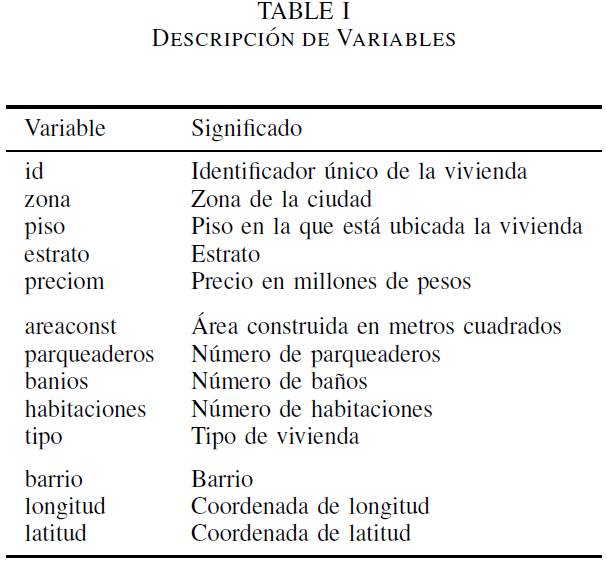
\includegraphics[width=0.7\linewidth]{images/Tabla1} \end{center}

Una vez se conocen las variables del conjunto de datos, procedemos a
identificar si son cuantitativas, cualitativas y categóricas.

\subsection{\textbf{Cuantitativas}}

Las variables cuantitavias son las siguientes:

\begin{center}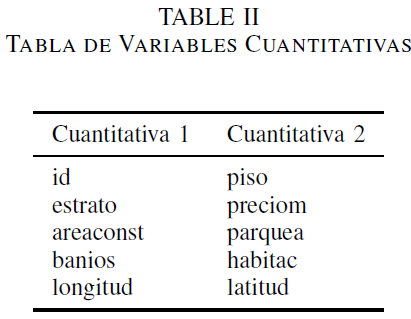
\includegraphics[width=0.6\linewidth]{images/Tabla2} \end{center}

\subsection{\textbf{Cualitativas}}

\begin{center}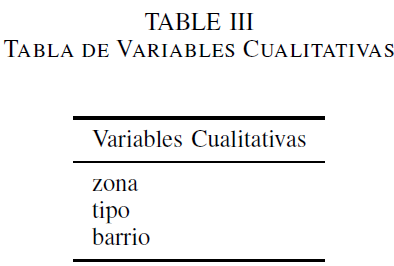
\includegraphics[width=0.6\linewidth]{images/Tabla3} \end{center}

Por otro lado, las anteriores variables cualitativas poseen las
siguientes categorías:

\subsection{\textbf{Categorías}}

\begin{center}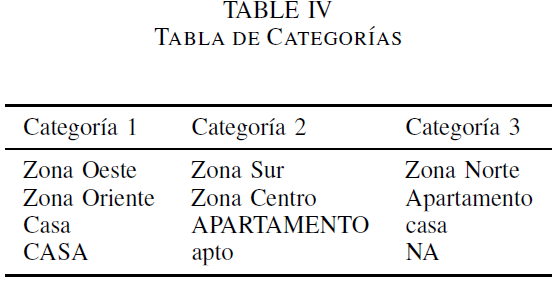
\includegraphics[width=0.8\linewidth]{images/Tabla4} \end{center}

\subsection{\textbf{Limpieza}}

A partir del conjunto de datos cargado, se procederá a realizar el
proceso de limpieza. Al haber observado las primeras 6 filas del
conjunto de datos, se pudo ver que hay una variedad de tipos de
propiedades, desde apartamentos hasta casas grandes, ubicadas en
diferentes zonas de la ciudad. Los precios y las áreas construidas
varían considerablemente.

\subsubsection{\textbf{Consideraciones para el análisis posterior}}

\begin{itemize}
\item
  Es importante notar que la variable zona y barrio pueden proporcionar
  información valiosa sobre la ubicación de las propiedades y su
  relación con el precio.
\item
  Las coordenadas geográficas (longitud y latitud) permiten realizar
  análisis espaciales.
\item
  Fue necesario identificar patrones y tendencias en los datos, como la
  relación entre el precio y el área construida, la distribución de los
  precios por zona, y la frecuencia de cada tipo de propiedad.
\end{itemize}

Primero calculamos la cantidad y el porcentaje de los datos faltantes
por columna:

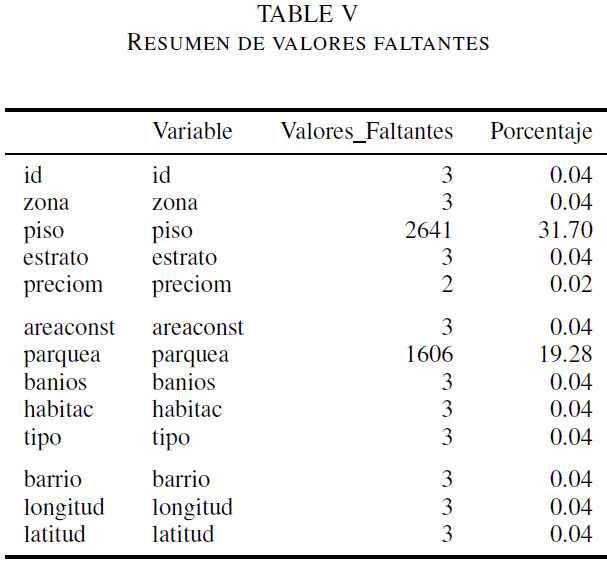
\includegraphics[width=0.9\linewidth]{images/Tabla5}

En base a lo anterior, podemos concluir lo siguiente:

\begin{itemize}
\item
  Las variables \textbf{\emph{``piso''}} y
  \textbf{\emph{``parqueaderos''}} presentan el mayor porcentaje de
  valores faltantes, con un \textbf{\emph{31.70\%}} y
  \textbf{\emph{19.27\%}} respectivamente, lo que requiere atención para
  evitar sesgos en el análisis.
\item
  El resto de las variables, como ``zona'', ``estrato'', ``preciom'',
  ``areaconst'', ``banios'', ``habitaciones'', ``tipo'', ``barrio'',
  ``longitud'' y ``latitud'', muestran un porcentaje mínimo de valores
  faltantes, todas por debajo del \textbf{\emph{0.04\%.}}.
\end{itemize}

Ahora para visualizar los patrones de datos faltantes y su relación con
otras variables, se utilizaron los gráficos
\ref{fig:dist-datos-faltantes-por-vars},
\ref{fig:grafico-barras-faltantes} y \ref{fig:grafico-barras-faltantes}:

\begin{center}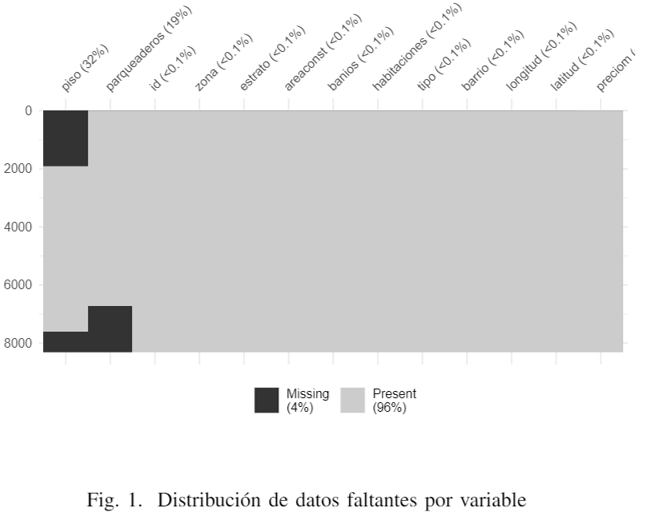
\includegraphics[width=1\linewidth]{images/ComparacionDatosFaltantesVariable} \end{center}

\begin{flushright}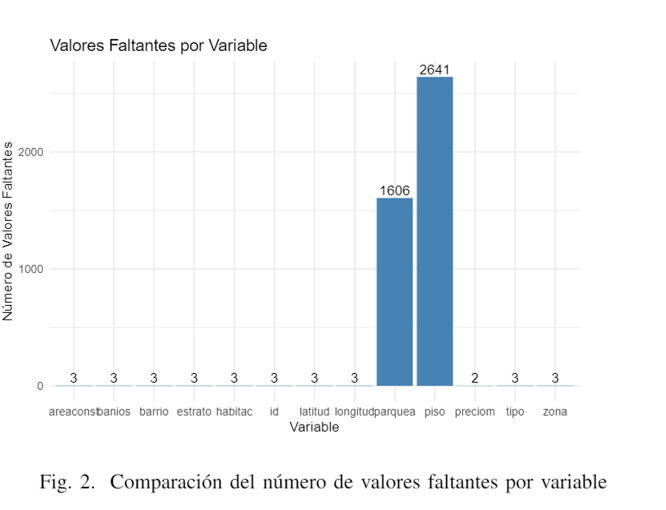
\includegraphics[width=1\linewidth]{images/GraficoBarrasFaltantes} \end{flushright}

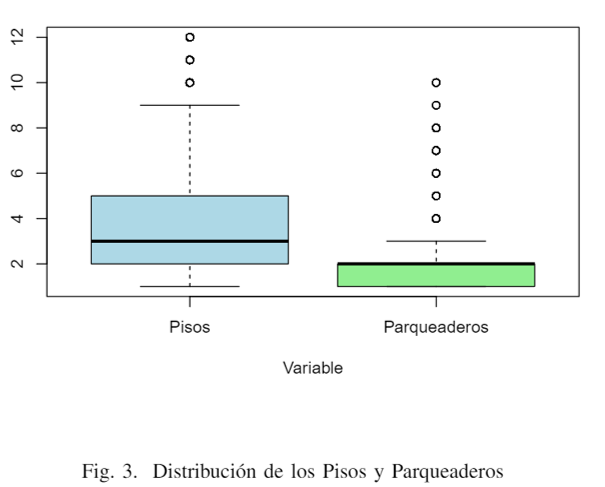
\includegraphics[width=1\linewidth]{images/BoxplotViviendaParqueadero}

\subsection{\textbf{Observaciones generales}}

\begin{itemize}
\item
  \textbf{Distribución de pisos y parqueaderos:} Tanto el número de
  pisos como el de parqueaderos presentan una distribución similar, con
  una ligera tendencia hacia valores más bajos. Esto indica que la
  mayoría de las viviendas tienen un número reducido de pisos y
  parqueaderos.
\item
  \textbf{Asimetría positiva:} La distribución de ambas variables
  muestra una leve asimetría positiva, lo que significa que hay una
  mayor concentración de datos en la parte inferior del rango, con una
  cola más larga hacia los valores más altos. Esto sugiere que existen
  algunas viviendas con un número significativamente mayor de pisos o
  parqueaderos.
\item
  \textbf{Mediana:} Comparando la mediana de parqueaderos (2) con el
  número promedio de vehículos por hogar en {[}zona{]}, se observa que,
  en promedio, las viviendas cuentan con un número de parqueaderos
  ligeramente inferior al número de vehículos. Esto sugiere que algunos
  hogares podrían tener más de un vehículo por vivienda.
\item
  \textbf{Valores atípicos:} Se observan valores atípicos en ambas
  variables, tanto en el extremo superior como en el inferior. Estos
  valores extremos podrían corresponder a viviendas con características
  inusuales, como edificios muy altos o casas muy pequeñas, o podrían
  ser el resultado de errores en la data.
\item
  \textbf{Dispersión:} A pesar de la presencia de valores atípicos, la
  dispersión de los datos, medida por el rango intercuartílico, es
  relativamente similar entre ambas variables. Esto sugiere que, en
  general, existe una variabilidad similar en el número de pisos y
  parqueaderos.
\end{itemize}

\subsection{\textbf{Frecuencia de tipos de vivienda}}

Si nos fijamos en los tipos de propiedades, vemos un pequeño error en
cuanto a la división de los tipos de vivienda, en donde se registraron
con diferentes nomenclaturas. Esto se aprecia a continuación:\\

\begin{flushleft}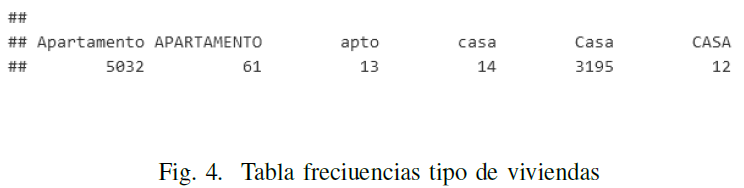
\includegraphics[width=1\linewidth]{images/FrecuenciaTiposViviendas} \end{flushleft}

\hfill\break
Lo anterior nos permite verificar que, después de la imputación de
datos, todas las categorías de tipo presentan una proporción de 0 en
valores faltantes para la variable `piso', lo que indica que se han
imputado correctamente todos los valores faltantes en esta columna,
eliminando cualquier NA y demostrando la efectividad del proceso de
imputación sin diferencias en la proporción de valores faltantes entre
los distintos tipos de propiedades.\\

Además, al analizar la relación entre los valores faltantes de `piso' y
el `tipo', la figura \ref{fig:bar-chart-proporcion-viviendas} revela que
la imputación ha sido exitosa en todas las categorías, consolidando la
ausencia de valores faltantes y asegurando la integridad de los datos en
la variable `piso'.

\begin{center}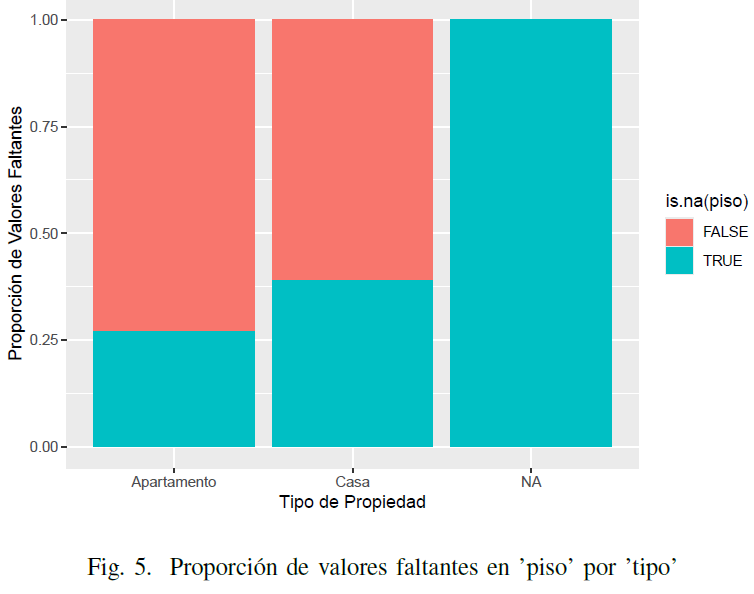
\includegraphics[width=1\linewidth]{images/ProporcionFaltantesPisoTipo} \end{center}

\subsection{\textbf{Barrio}}

La variable barrio será modificada iniciando con el cambio del texto a
minúscula, remoción de tildes y posteriomente el reemplazo de valores en
las categorías donde existan nombres similares. El cambio se ve a
continuación, la cantidad de barrios pasa de 436 a 370.\\

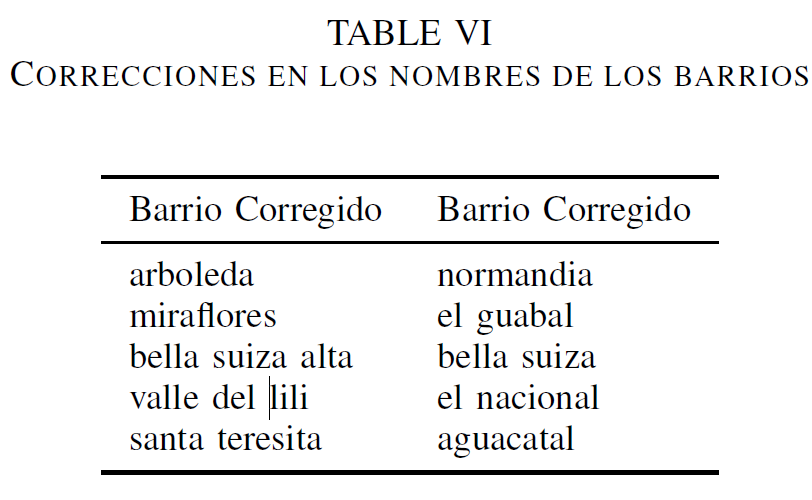
\includegraphics[width=0.8\linewidth]{images/Tabla6}

\subsection{\textbf{Eliminación de valores NA}}

Se decide eliminar los valores NA de todas las variables, menos las de
las columnas de `parqueadero' y `piso' al representar un alto porcentaje
de datos faltantes en comparación con las demás. Teniendo en cuenta lo
previo, se puede visualizar que los 3 registros no contienen información
en ninguna de sus 13 variables por lo que serán eliminados. A
continuación, se muestra nuevamente la tabla de los valores NA.

\begin{center}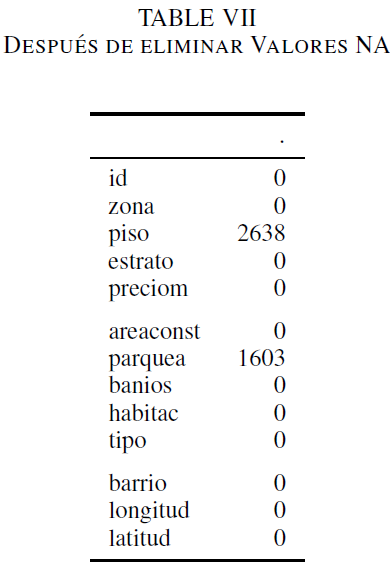
\includegraphics[width=0.5\linewidth]{images/Table7} \end{center}

\subsection{\textbf{Visualización}}

En esta etapa, nos enfocaremos en dar respuesta a los objetivos
propuestos al inicio. Para ello, haremos uso de gráficos que permitan
visualizar la información.

\subsection{\textbf{¿Cuál es el precio de las viviendas en diferentes zonas?}}

En este caso se agregó la variable precio por metro cuadrado
(precio\_m2) a la base para usarla dentro del análisis. Adicionalmente,
se dividirá la visualización en 3 secciones por la variable tipo:
apartamento y casa, casa y apartamento.\\

\subsubsection{\textbf{Apartamento y casa}}

\hfill\break
El mapa que se muestra a continuación permite observar la distribución
del precio por zonas teniendo en cuenta casas y apartamentos.

\begin{center}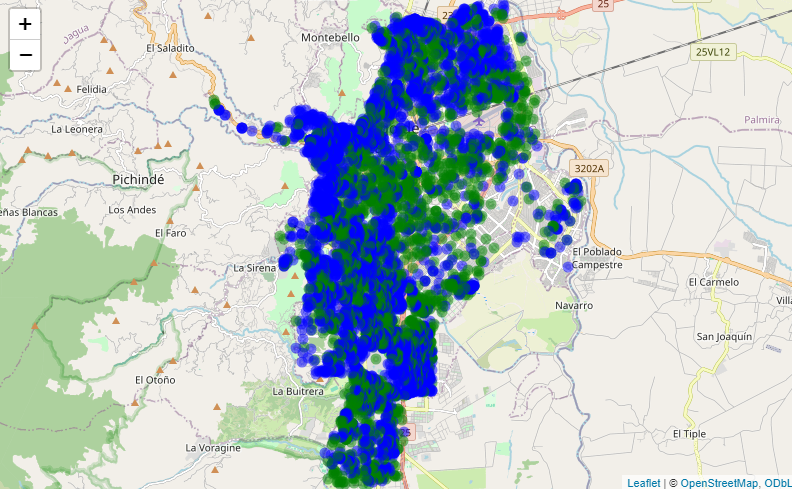
\includegraphics[width=0.8\linewidth]{images/Map} \end{center}

La siguiente tabla muestra los valores del promedio y la mediana para
las variables precio y precio por metro cuadrado de casas y
apartamentos.

\begin{center}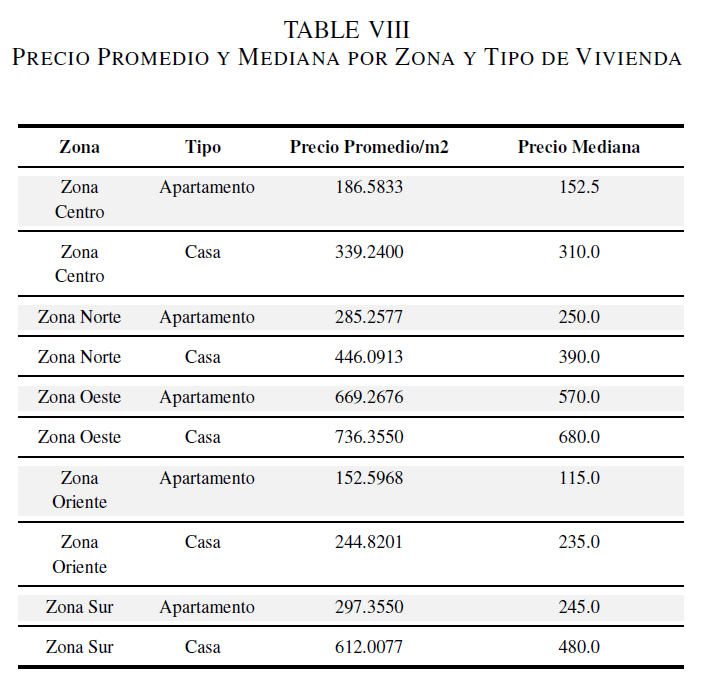
\includegraphics[width=0.9\linewidth]{images/Table8} \end{center}

\subsection{\textbf{¿Cuál es el tipo de vivienda más ofertada?}}

A continuación, en la figura \ref{fig:pie-chart-viviendas} se usa un
gráfico de tipo torta o pie para visualizar la distribución de los tipos
de viviendas en Cali.

\begin{flushright}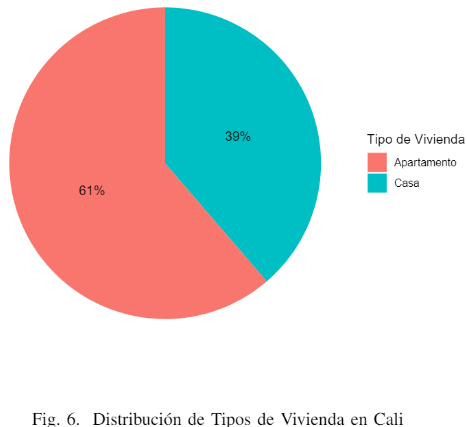
\includegraphics[width=0.9\linewidth]{images/pie-chart-viviendas} \end{flushright}
\subsection{\textbf{¿Cuáles son las características más relevantes?}}

\textbf{1. Precio y precio por metro cuadrado}\\
A continuación, se comparan las variables precio (preciom) y precio por
metro cuadrado (precio\_m2) usando un gráfico de cajas.\newpage

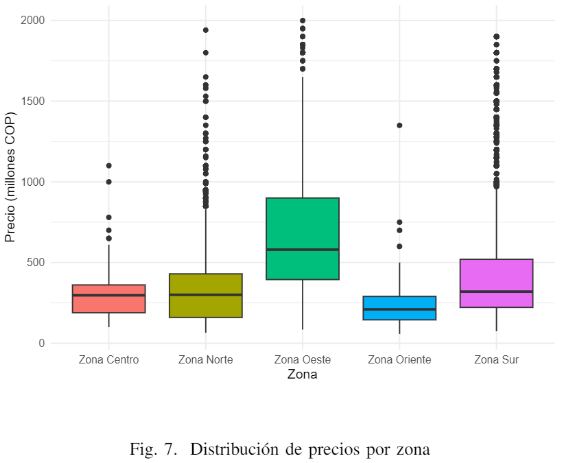
\includegraphics[width=1\linewidth]{images/BoxplotPreciosZona}

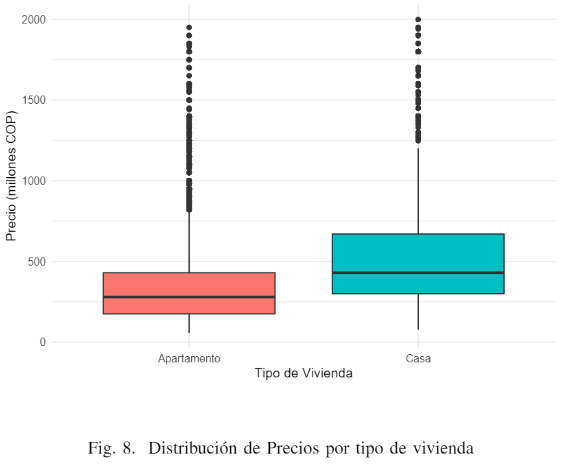
\includegraphics[width=1\linewidth]{images/BoxplotPreciosTipo}

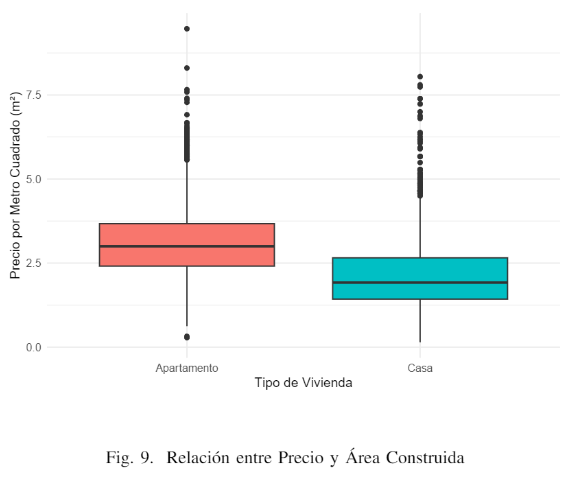
\includegraphics[width=1\linewidth]{images/BoxplotPreciosArea}

\textbf{2. Precio por zona}\\
Por otro lado, se realizó un gráfico de barras para poder comparar la
distribución de los tipos de viviendas y sus características propias:

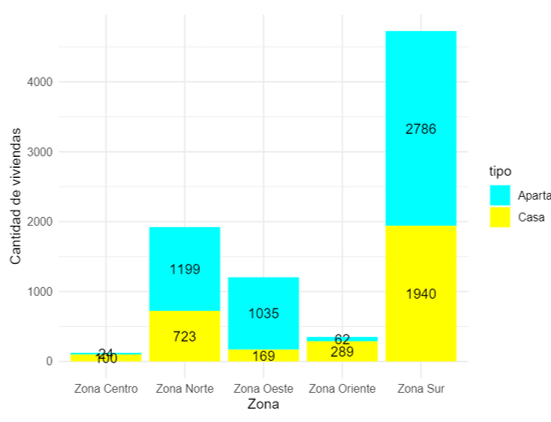
\includegraphics[width=1\linewidth]{images/PrecioPorZona}

\textbf{3. Viviendas por Piso}\\

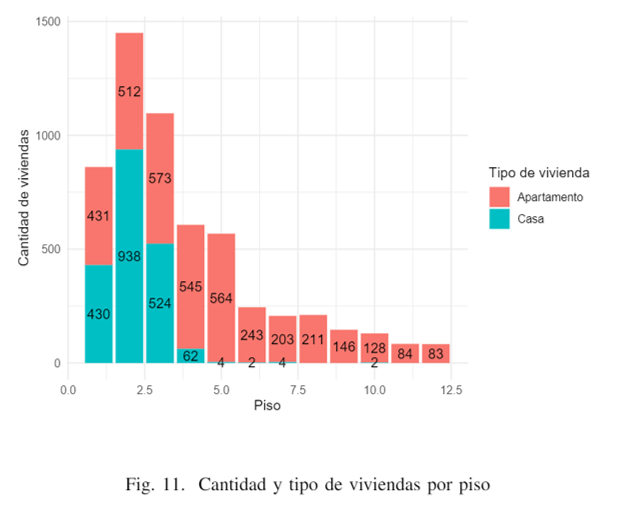
\includegraphics[width=1\linewidth]{images/CantTipoPorPiso}

\textbf{Análisis por Área Construida}\\
Para este análisis usamos un diagrama de tipo histograma

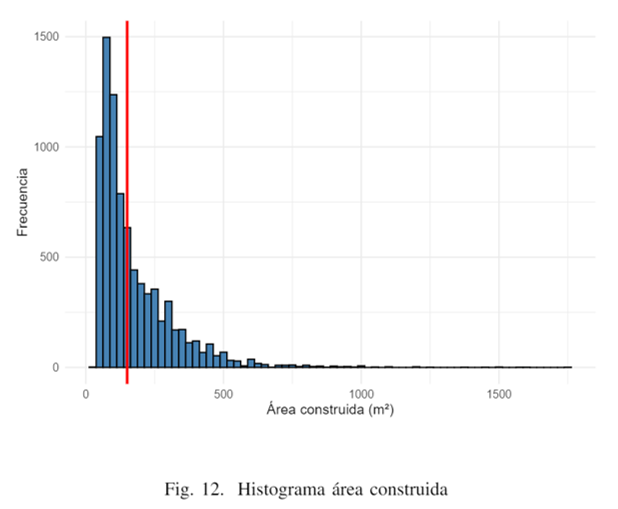
\includegraphics[width=1\linewidth]{images/HistogramaAreaConst}

\textbf{Habitaciones}\\
Ahora veremos la información relacionada con las habitaciones

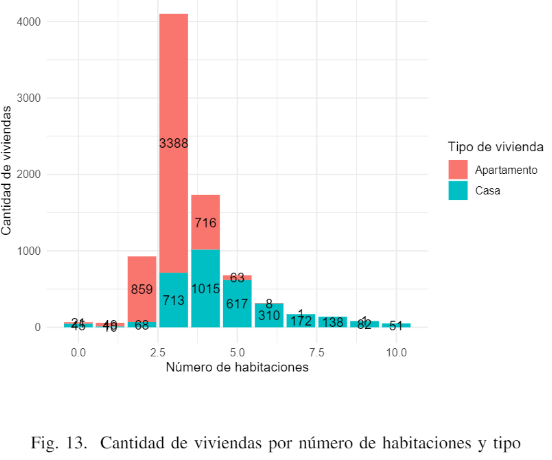
\includegraphics[width=1\linewidth]{images/HabitacionesPorTipo}
\textbf{Estrato}\\
A continuación, veremos la información relacionada con la variable
estrato.

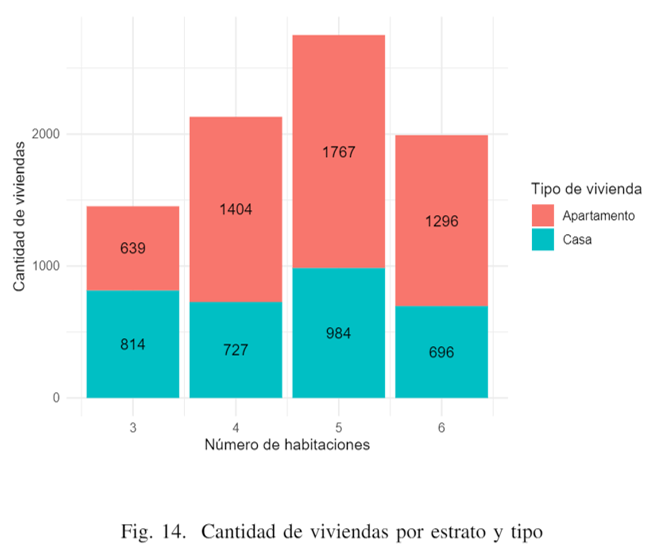
\includegraphics[width=1\linewidth]{images/EstratoHabitacionesPorTipo}

\textbf{Número de parqueaderos}\\
Ahora veremos la información relacionada con el número de parqueaderos.

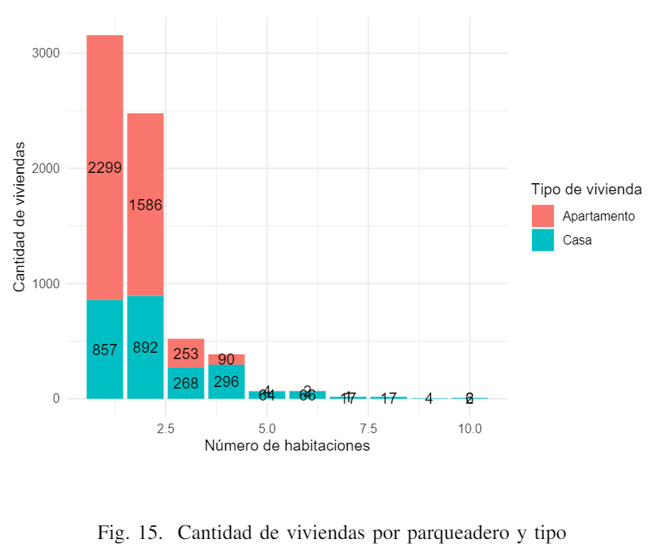
\includegraphics[width=1\linewidth]{images/ParqueaderosPorTipo}

\textbf{Baños}\\
Ahora veremos la información relacionada con la cantidad de baños.

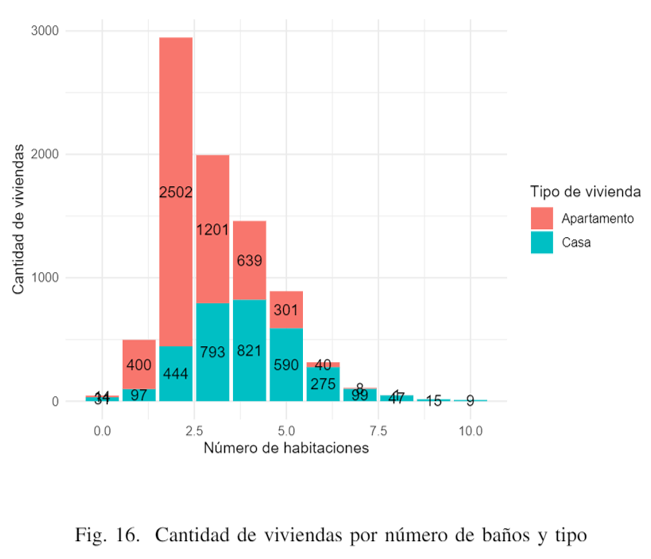
\includegraphics[width=1\linewidth]{images/BaniosPorTipo}

\textbf{Análisis de correlación}\\
Calcularemos una matriz de correlación para identificar las variables
que están más fuertemente relacionadas con el precio

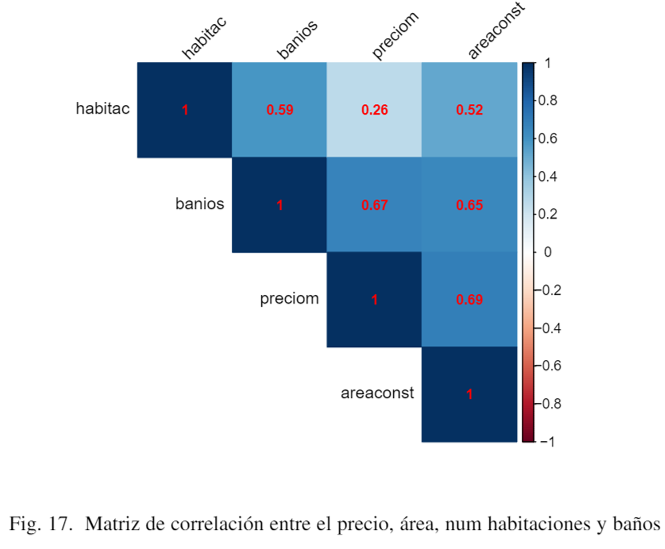
\includegraphics[width=1\linewidth]{images/MatrizCorrelacion}

De lo anterior, se puede decir que la correlación entre:

\begin{enumerate}
\def\labelenumi{\arabic{enumi}.}
\item
  \textbf{Precio y Área Construida:} El coeficiente de correlación de
  0.687 muestra una relación positiva fuerte, indicando que, en general,
  propiedades más grandes tienen precios más altos.
\item
  \textbf{Precio y Número de Habitaciones:} El coeficiente de 0.263
  sugiere una relación positiva moderada, pero menos intensa que la
  observada entre el precio y el área construida.
\item
  \textbf{Área Construida y Número de Habitaciones:} El coeficiente de
  0.517 indica una relación positiva moderada, lo cual es lógico ya que
  propiedades más grandes tienden a tener más habitaciones.
\item
  \textbf{Precio y Número de Baños:} Existe una correlación positiva
  fuerte entre el precio y el número de baños. Esto indica que
  propiedades con más baños tienden a tener precios más altos.
\end{enumerate}

\subsection{\textbf{Nicho de mercado}}

Para respaldar la toma de decisiones en relación con el nicho de
mercado, se llevará a cabo un análisis separado según el tipo de
vivienda. Además, el nicho de mercado está estrechamente vinculado con
las ventas y, por ende, con el precio. En este contexto, las principales
variables de análisis serán el precio y el precio por metro cuadrado.
Las variables adicionales a considerar incluirán aspectos relacionados
con la venta o características del inmueble que influyen en el cliente,
tales como la \textbf{zona y el estrato.} La variable barrio no se
incluirá debido a la gran cantidad de valores únicos.\\

\newpage

\textbf{Apartamentos}\\

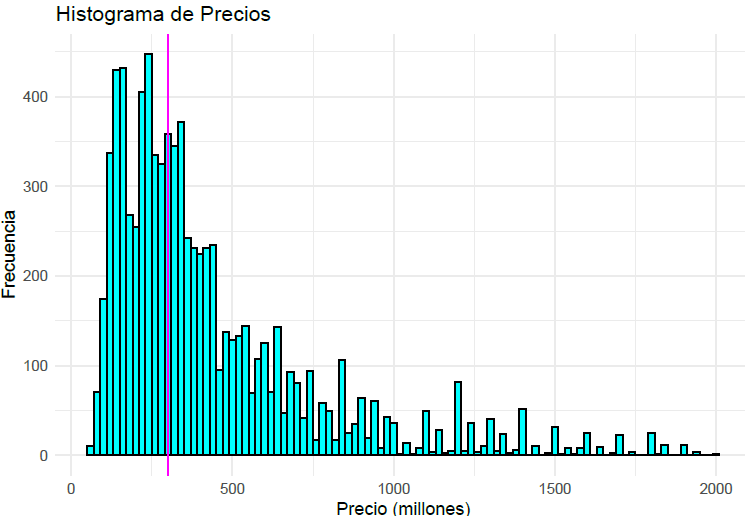
\includegraphics[width=1\linewidth]{images/HistogramaPrecios}

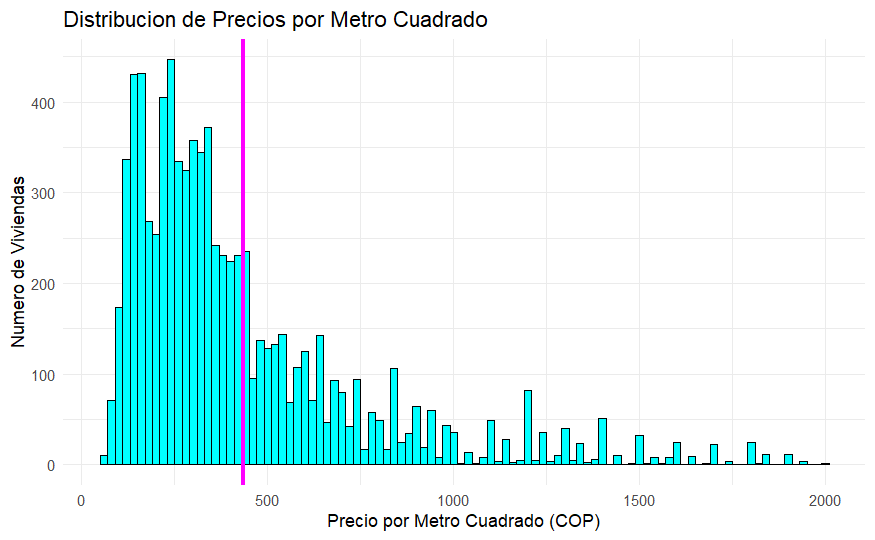
\includegraphics[width=1\linewidth]{images/DistrPreciosMetroCuadrado}

\section{IV. Resultados}

A continuación se listan los resultados basados en el ejercicio de
visualización de la sección anterior:

\subsection{\textbf{Información sobre precio de viviendas}}

El precio promedio del costo total y costo por metro cuadrado de las
viviendas en diferentes zonas de Cali, teniendo en cuenta \textbf{ambos
tipos de vivienda}, es:\\

\begin{itemize}
\tightlist
\item
  Zona Centro: 310 millones, 1,75 millones/m\^{}2
\item
  Zona Norte: 346 millones, 2,45 millones/m\^{}2
\item
  Zona Oeste: 679 millones, 3,65 millones/m\^{}2
\item
  Zona Oriente: 229 millones, 1,44 millones/m\^{}2
\item
  Zona Sur: 426 millones, 2,72 millones/m\^{}2
\end{itemize}

El precio promedio del costo total y costo por metro cuadrado de las
viviendas en diferentes zonas de Cali, teniendo en cuenta solo los
\textbf{apartamentos}, es:\\

\begin{itemize}
\tightlist
\item
  Zona Centro: 187 millones, 1,95 millones/m\^{}2
\item
  Zona Norte: 285 millones, 2,81 millones/m\^{}2
\item
  Zona Oeste: 669 millones, 3,85 millones/m\^{}2
\item
  Zona Oriente: 153 millones, 1,69 millones/m\^{}2
\item
  Zona Sur: 297 millones, 2,98 millones/m\^{}2
\end{itemize}

El precio promedio del costo total y costo por metro cuadrado de las
viviendas en diferentes zonas de Cali, teniendo en cuenta solo las
casas, es:\\

\begin{itemize}
\tightlist
\item
  Zona Centro: 339 millones, 1,69 millones/m\^{}2
\item
  Zona Norte: 446 millones, 1,84 millones/m\^{}2
\item
  Zona Oeste: 736 millones, 2,38 millones/m\^{}2
\item
  Zona Oriente: 244 millones, 1,38 millones/m\^{}2
\item
  Zona Sur: 612 millones, 2,33 millones/m\^{}2
\end{itemize}

\subsection{\textbf{Tipo de vivienda más ofertada}}

El tipo de vivienda más ofertada en Cali es: - Apartamento: 61\% - Casa:
39\%

\subsection{\textbf{Caracteristicas relevantes}}

\begin{itemize}
\tightlist
\item
  \textbf{Precio:} además de los resultados del precio mencionados
  anteriomente, la distribución del precio en millones de apartamentos
  se encuentra por encima cuando se evalua teniendo en cuenta el área
  construida.
\item
  \textbf{Zona:} la zona sur, norte y oeste tienen la mayor proporción
  de oferta de viviendas.
\item
  \textbf{Piso:} las casas y apartamentos tienen proporciones similares
  de piso 1-3. A partir de piso 4 la participación de los apartamentos
  se lleva la mayor proporción.
\item
  \textbf{Área construida:} la variable se distribuye principalmente
  entre 0 y 400 metros cuadrados, la mediana es 123 metros cuadrados.
\item
  \textbf{Número de habitaciones:} la variable tiene mayor participación
  de apartamentos entre 0-3 habitaciones, a partir de 4 la participación
  es mayor en casas.
\item
  \textbf{Estrato:} el estrato 5 se lleva la mayor proporción de oferta
  de vivienda teniendo más participación de apartamentos que de casas.
\item
  \textbf{Número de parqueaderos:} De 1 a 3 parqueaderos tiene la mayor
  proporción de oferta de vivienda teniendo más participación de
  apartamentos que de casas. A partir de 4 parqueaderos las casas tienen
  más participación.
\item
  \textbf{Baños:} De 1 a 3 baños tiene la mayor proporción de oferta de
  vivienda teniendo más participación de apartamentos que de casas. A
  partir de 4 baños las casas tienen más participación.
\end{itemize}

\subsection{\textbf{Nicho de mercado}}

\textbf{Apartamento}\newline - \textbf{Precio:} el precio por metro
cuadrado se podría ubicar entre 1 y 2 millones o entre 4 y 6 millones.\\
- \textbf{Zona:} la zona podría estar en norte o en oeste/sur.\\
- \textbf{Estrato:} el estrato podría estar en 3 o 5-6.\\
- \textbf{Precio:} el precio por metro cuadrado se podría ubicar entre 0
y 1 millones o entre 3 y 5 millones.\\
- \textbf{Zona}: la zona podría estar en oriente o en oeste/sur.\\
- \textbf{Estrato}:el estrato podría estar en 3 o 5-6.\\

\section{\textbf{Nicho de mercado}}

\subsection{\textbf{Información de precio}}

La información sobre los precios de las viviendas en Cali se puede
analizar considerando ambos tipos de propiedad: apartamentos y casas. En
el caso de los apartamentos, las zonas oeste y sur presentan los valores
promedio más altos, con 3,65 y 2,72 millones por metro cuadrado,
respectivamente. Para los apartamentos, las zonas oeste y sur siguen
destacándose con promedios de 3,85 y 2,98 millones por metro cuadrado,
aunque la zona norte está bastante cerca, con 2,81 millones por metro
cuadrado. En cuanto a las casas, las zonas oeste y sur mantienen el
mismo patrón, con promedios de 2,38 y 2,33 millones por metro cuadrado.

\subsection{\textbf{Tipo de vivivenda más ofertada}}

El tipo de vivienda con mayor participación en el mercado de Cali es el
apartamento, que representa el 61\% de la oferta, mientras que las casas
constituyen el 39\%.

\subsection{\textbf{Características a destacar}}

\begin{enumerate}
\def\labelenumi{\arabic{enumi}.}
\item
  El análisis del precio por metro cuadrado ofrece una visión más clara
  del costo de la vivienda. Aunque las casas tienen un precio
  globalmente más alto sin considerar el área, al evaluar el precio por
  metro cuadrado, se observa que el 75\% de los datos de apartamentos se
  sitúa cerca de 4 millones por metro cuadrado, mientras que el mismo
  porcentaje para las casas está alrededor de 3 millones por metro
  cuadrado.
\item
  Las zonas sur, norte y oeste presentan la mayor proporción de oferta
  de vivienda, con el 56\%, 23\% y 14\%, respectivamente. El patrón de
  pisos de las casas, que usualmente tienen de 1 a 3 pisos, contrasta
  con los apartamentos, que predominan en edificios y, por lo tanto,
  tienen una mayor participación en el mercado.
\item
  Para el área construida, se utilizó la mediana debido a la presencia
  de valores extremos. Esta área varía entre 0 y 400 metros cuadrados, y
  dado que los apartamentos tienen una mayor proporción, es consistente
  que su mediana sea de 123 metros cuadrados. El número de habitaciones,
  baños y parqueaderos sigue una tendencia similar, con una mayor
  proporción en apartamentos de 1 a 3 habitaciones, 1 a 3 baños y 1 a 3
  parqueaderos. Finalmente, el estrato 5 es el más representado en el
  mercado, dado que la variable está entre los estratos 3 y 6, sin
  presencia de los estratos 1 y 2.
\end{enumerate}

\subsection{\textbf{Nicho a enfocar}}

onsiderando la información de la base de datos y el concepto de nicho de
mercado de HubSpot, el nicho de mercado se define como una parte del
segmento de mercado que no ha sido completamente explorada pero que ha
realizado compras en el pasado. Por lo tanto, se sugiere a B\&C (Bines y
Casas) enfocarse en los siguientes nichos de mercado:

\textbf{Apartamento}

\begin{enumerate}
\def\labelenumi{\arabic{enumi}.}
\tightlist
\item
  \textbf{Enfoque 1: Menor Precio por Metro Cuadrado}
\end{enumerate}

\begin{itemize}
\tightlist
\item
  Precio: Entre 1 y 2 millones por metro cuadrado.
\item
  Zona: Norte.
\item
  Estrato: 3.
\item
  Comentario: Este enfoque está dirigido a nichos con menor capacidad de
  compra, incluyendo programas de vivienda de interés social (VIS)
  ajustados a los topes salariales vigentes.
\end{itemize}

\begin{enumerate}
\def\labelenumi{\arabic{enumi}.}
\setcounter{enumi}{1}
\tightlist
\item
  \textbf{Enfoque 2: Mayor Precio por Metro Cuadrado}
\end{enumerate}

\begin{itemize}
\tightlist
\item
  Precio: Entre 4 y 6 millones por metro cuadrado.
\item
  Zona: Oeste o Sur.
\item
  Estrato: 5 o 6.
\item
  Comentario: Este enfoque está dirigido a nichos con mayor capacidad de
  compra.
\end{itemize}

\textbf{Casa}

\begin{enumerate}
\def\labelenumi{\arabic{enumi}.}
\tightlist
\item
  \textbf{Enfoque 1: Menor Precio por Metro Cuadrado}
\end{enumerate}

\begin{itemize}
\tightlist
\item
  Precio: Entre 0 y 1 millón por metro cuadrado.
\item
  Zona: Oriente.
\item
  Estrato: 3.
\item
  Comentario: Este enfoque está orientado a nichos con menor capacidad
  de compra.
\end{itemize}

\begin{enumerate}
\def\labelenumi{\arabic{enumi}.}
\setcounter{enumi}{1}
\tightlist
\item
  \textbf{Enfoque 2: Mayor Precio por Metro Cuadrado}
\end{enumerate}

\begin{itemize}
\tightlist
\item
  Precio: Entre 3 y 5 millones por metro cuadrado.
\item
  Zona: Oeste o Sur.
\item
  Estrato: 5 o 6.
\item
  Comentario: Este enfoque está dirigido a nichos con mayor capacidad de
  compra.
\end{itemize}

\subsection{\textbf{Estrategias de marketing}}

La creación de estrategias de marketing puede optimizarse mediante el
desarrollo de arquetipos o buyer personas. En este sentido, se sugiere
lo siguiente:

\textbf{Para los apartamentos:}

\begin{itemize}
\tightlist
\item
  Buyer Persona: Parejas sin hijos con una alta capacidad de compra
  conjunta.
\item
  Características: Profesionales de entre 28 y 40 años, con mascotas,
  que prefieren vivir en zonas cercanas a centros comerciales o de
  oficinas.
\end{itemize}

\textbf{Para las casas:}

\begin{itemize}
\tightlist
\item
  \textbf{Buyer Persona:} Parejas con uno o más hijos, mayores de 30
  años.
\item
  \textbf{Características:* }Se recomienda obtener información
  financiera detallada de los clientes para crear audiencias
  personalizadas en plataformas de anuncios. Con esta información, se
  pueden buscar personas similares, utilizando, por ejemplo, audiencias
  de eventos importantes en Google que estén interesadas en bienes
  raíces.\\
\end{itemize}

Por otra parte, los precios de venta recomendados se basan en las
características del nicho de mercado identificado. Es importante
destacar que:

\begin{itemize}
\tightlist
\item
  Para los apartamentos: La mediana del precio es de 3 millones por
  metro cuadrado y 280 millones por unidad.
\item
  Para las casas: La mediana del precio es de 1,92 millones por metro
  cuadrado y 430 millones por unidad.
\end{itemize}

\section{\textbf{V. Conclusiones}}

La información sobre los precios de las viviendas en Cali se puede
analizar considerando ambos tipos de propiedad: apartamentos y casas. En
la zona oeste, el costo promedio es de 3,65 millones por metro cuadrado
tanto para casas como para apartamentos. Sin embargo, para los
apartamentos, el costo promedio en esta zona es de 3,85 millones por
metro cuadrado, mientras que para las casas es de 2,38 millones por
metro cuadrado.\\

El tipo de vivienda más ofertado es el apartamento, con una
participación del 61\% del total.\\

\textbf{Sugerencias para el Nicho de Mercado:}

\begin{enumerate}
\def\labelenumi{\arabic{enumi}.}
\tightlist
\item
  \textbf{Para apartamentos:}
\end{enumerate}

\begin{itemize}
\tightlist
\item
  Precio por metro cuadrado: Entre 1 y 2 millones o entre 4 y 6
  millones.
\item
  Zona: Norte o oeste/sur.
\item
  Estrato: 3 o 5-6, según el enfoque comercial.
\end{itemize}

\begin{enumerate}
\def\labelenumi{\arabic{enumi}.}
\setcounter{enumi}{1}
\tightlist
\item
  \textbf{Para casas:}
\end{enumerate}

\begin{itemize}
\tightlist
\item
  Precio por metro cuadrado: Entre 0 y 1 millón o entre 3 y 5 millones.
\item
  Zona: Oriente o oeste/sur.
\item
  Estrato: 3 o 5-6, según el enfoque comercial.
\end{itemize}

\begin{enumerate}
\def\labelenumi{\arabic{enumi}.}
\setcounter{enumi}{2}
\tightlist
\item
  \textbf{Precios de Venta del Segmento de Mercado:}
\end{enumerate}

-Apartamentos: La mediana es de 3 millones por metro cuadrado y 280
millones por unidad. - Casas: La mediana es de 1,92 millones por metro
cuadrado y 430 millones por unidad.

\section{REFERENCIAS}\label{references}

{[}1{]} M. F. Meneses-González and C. E. Sánchez, ``Informe especial de
Estabilidad Financiera: Análisis de la Cartera y del mercado
inmobiliario en colombia - segundo semestre de 2023,'' DSpace,
https://repositorio.banrep.gov.co/items/baf87440-d6ad-402c-adb4-d7a3e3f241c0/

{[}2{]} G. V. Richard, ``Caracterización de estrategias de marketing
digital, en el sector inmobiliario de Cali,'' Red UAO Home, Sep.~06,
2023.
https://red.uao.edu.co/entities/publication/1d0b24eb-420a-4a13-8ae2-81f8faf1ebd6

{[}3{]} M. F. Meneses and C. E. Sánchez, ``Análisis de la cartera y del
mercado inmobiliario en Colombia,'' INFORME ESPECIAL, Jul.~2023,
{[}Online{]}. Available:
https://web.archive.org/web/20240122113855id\_/https://repositorio.banrep.gov.co/bitstream/handle/20.500.12134/10755/Informe\_Especial\_vivienda\_2023-II.pdf

\end{document}

